% Options for packages loaded elsewhere
% Options for packages loaded elsewhere
\PassOptionsToPackage{unicode}{hyperref}
\PassOptionsToPackage{hyphens}{url}
\PassOptionsToPackage{dvipsnames,svgnames,x11names}{xcolor}
%
\documentclass[
  letterpaper,
  DIV=11,
  numbers=noendperiod]{scrartcl}
\usepackage{xcolor}
\usepackage{amsmath,amssymb}
\setcounter{secnumdepth}{-\maxdimen} % remove section numbering
\usepackage{iftex}
\ifPDFTeX
  \usepackage[T1]{fontenc}
  \usepackage[utf8]{inputenc}
  \usepackage{textcomp} % provide euro and other symbols
\else % if luatex or xetex
  \usepackage{unicode-math} % this also loads fontspec
  \defaultfontfeatures{Scale=MatchLowercase}
  \defaultfontfeatures[\rmfamily]{Ligatures=TeX,Scale=1}
\fi
\usepackage{lmodern}
\ifPDFTeX\else
  % xetex/luatex font selection
\fi
% Use upquote if available, for straight quotes in verbatim environments
\IfFileExists{upquote.sty}{\usepackage{upquote}}{}
\IfFileExists{microtype.sty}{% use microtype if available
  \usepackage[]{microtype}
  \UseMicrotypeSet[protrusion]{basicmath} % disable protrusion for tt fonts
}{}
\makeatletter
\@ifundefined{KOMAClassName}{% if non-KOMA class
  \IfFileExists{parskip.sty}{%
    \usepackage{parskip}
  }{% else
    \setlength{\parindent}{0pt}
    \setlength{\parskip}{6pt plus 2pt minus 1pt}}
}{% if KOMA class
  \KOMAoptions{parskip=half}}
\makeatother
% Make \paragraph and \subparagraph free-standing
\makeatletter
\ifx\paragraph\undefined\else
  \let\oldparagraph\paragraph
  \renewcommand{\paragraph}{
    \@ifstar
      \xxxParagraphStar
      \xxxParagraphNoStar
  }
  \newcommand{\xxxParagraphStar}[1]{\oldparagraph*{#1}\mbox{}}
  \newcommand{\xxxParagraphNoStar}[1]{\oldparagraph{#1}\mbox{}}
\fi
\ifx\subparagraph\undefined\else
  \let\oldsubparagraph\subparagraph
  \renewcommand{\subparagraph}{
    \@ifstar
      \xxxSubParagraphStar
      \xxxSubParagraphNoStar
  }
  \newcommand{\xxxSubParagraphStar}[1]{\oldsubparagraph*{#1}\mbox{}}
  \newcommand{\xxxSubParagraphNoStar}[1]{\oldsubparagraph{#1}\mbox{}}
\fi
\makeatother

\usepackage{color}
\usepackage{fancyvrb}
\newcommand{\VerbBar}{|}
\newcommand{\VERB}{\Verb[commandchars=\\\{\}]}
\DefineVerbatimEnvironment{Highlighting}{Verbatim}{commandchars=\\\{\}}
% Add ',fontsize=\small' for more characters per line
\usepackage{framed}
\definecolor{shadecolor}{RGB}{241,243,245}
\newenvironment{Shaded}{\begin{snugshade}}{\end{snugshade}}
\newcommand{\AlertTok}[1]{\textcolor[rgb]{0.68,0.00,0.00}{#1}}
\newcommand{\AnnotationTok}[1]{\textcolor[rgb]{0.37,0.37,0.37}{#1}}
\newcommand{\AttributeTok}[1]{\textcolor[rgb]{0.40,0.45,0.13}{#1}}
\newcommand{\BaseNTok}[1]{\textcolor[rgb]{0.68,0.00,0.00}{#1}}
\newcommand{\BuiltInTok}[1]{\textcolor[rgb]{0.00,0.23,0.31}{#1}}
\newcommand{\CharTok}[1]{\textcolor[rgb]{0.13,0.47,0.30}{#1}}
\newcommand{\CommentTok}[1]{\textcolor[rgb]{0.37,0.37,0.37}{#1}}
\newcommand{\CommentVarTok}[1]{\textcolor[rgb]{0.37,0.37,0.37}{\textit{#1}}}
\newcommand{\ConstantTok}[1]{\textcolor[rgb]{0.56,0.35,0.01}{#1}}
\newcommand{\ControlFlowTok}[1]{\textcolor[rgb]{0.00,0.23,0.31}{\textbf{#1}}}
\newcommand{\DataTypeTok}[1]{\textcolor[rgb]{0.68,0.00,0.00}{#1}}
\newcommand{\DecValTok}[1]{\textcolor[rgb]{0.68,0.00,0.00}{#1}}
\newcommand{\DocumentationTok}[1]{\textcolor[rgb]{0.37,0.37,0.37}{\textit{#1}}}
\newcommand{\ErrorTok}[1]{\textcolor[rgb]{0.68,0.00,0.00}{#1}}
\newcommand{\ExtensionTok}[1]{\textcolor[rgb]{0.00,0.23,0.31}{#1}}
\newcommand{\FloatTok}[1]{\textcolor[rgb]{0.68,0.00,0.00}{#1}}
\newcommand{\FunctionTok}[1]{\textcolor[rgb]{0.28,0.35,0.67}{#1}}
\newcommand{\ImportTok}[1]{\textcolor[rgb]{0.00,0.46,0.62}{#1}}
\newcommand{\InformationTok}[1]{\textcolor[rgb]{0.37,0.37,0.37}{#1}}
\newcommand{\KeywordTok}[1]{\textcolor[rgb]{0.00,0.23,0.31}{\textbf{#1}}}
\newcommand{\NormalTok}[1]{\textcolor[rgb]{0.00,0.23,0.31}{#1}}
\newcommand{\OperatorTok}[1]{\textcolor[rgb]{0.37,0.37,0.37}{#1}}
\newcommand{\OtherTok}[1]{\textcolor[rgb]{0.00,0.23,0.31}{#1}}
\newcommand{\PreprocessorTok}[1]{\textcolor[rgb]{0.68,0.00,0.00}{#1}}
\newcommand{\RegionMarkerTok}[1]{\textcolor[rgb]{0.00,0.23,0.31}{#1}}
\newcommand{\SpecialCharTok}[1]{\textcolor[rgb]{0.37,0.37,0.37}{#1}}
\newcommand{\SpecialStringTok}[1]{\textcolor[rgb]{0.13,0.47,0.30}{#1}}
\newcommand{\StringTok}[1]{\textcolor[rgb]{0.13,0.47,0.30}{#1}}
\newcommand{\VariableTok}[1]{\textcolor[rgb]{0.07,0.07,0.07}{#1}}
\newcommand{\VerbatimStringTok}[1]{\textcolor[rgb]{0.13,0.47,0.30}{#1}}
\newcommand{\WarningTok}[1]{\textcolor[rgb]{0.37,0.37,0.37}{\textit{#1}}}

\usepackage{longtable,booktabs,array}
\usepackage{calc} % for calculating minipage widths
% Correct order of tables after \paragraph or \subparagraph
\usepackage{etoolbox}
\makeatletter
\patchcmd\longtable{\par}{\if@noskipsec\mbox{}\fi\par}{}{}
\makeatother
% Allow footnotes in longtable head/foot
\IfFileExists{footnotehyper.sty}{\usepackage{footnotehyper}}{\usepackage{footnote}}
\makesavenoteenv{longtable}
\usepackage{graphicx}
\makeatletter
\newsavebox\pandoc@box
\newcommand*\pandocbounded[1]{% scales image to fit in text height/width
  \sbox\pandoc@box{#1}%
  \Gscale@div\@tempa{\textheight}{\dimexpr\ht\pandoc@box+\dp\pandoc@box\relax}%
  \Gscale@div\@tempb{\linewidth}{\wd\pandoc@box}%
  \ifdim\@tempb\p@<\@tempa\p@\let\@tempa\@tempb\fi% select the smaller of both
  \ifdim\@tempa\p@<\p@\scalebox{\@tempa}{\usebox\pandoc@box}%
  \else\usebox{\pandoc@box}%
  \fi%
}
% Set default figure placement to htbp
\def\fps@figure{htbp}
\makeatother





\setlength{\emergencystretch}{3em} % prevent overfull lines

\providecommand{\tightlist}{%
  \setlength{\itemsep}{0pt}\setlength{\parskip}{0pt}}



 


\usepackage{fvextra}
\DefineVerbatimEnvironment{Highlighting}{Verbatim}{breaklines,breakanywhere}
\KOMAoption{captions}{tableheading}
\makeatletter
\@ifpackageloaded{caption}{}{\usepackage{caption}}
\AtBeginDocument{%
\ifdefined\contentsname
  \renewcommand*\contentsname{Table of contents}
\else
  \newcommand\contentsname{Table of contents}
\fi
\ifdefined\listfigurename
  \renewcommand*\listfigurename{List of Figures}
\else
  \newcommand\listfigurename{List of Figures}
\fi
\ifdefined\listtablename
  \renewcommand*\listtablename{List of Tables}
\else
  \newcommand\listtablename{List of Tables}
\fi
\ifdefined\figurename
  \renewcommand*\figurename{Figure}
\else
  \newcommand\figurename{Figure}
\fi
\ifdefined\tablename
  \renewcommand*\tablename{Table}
\else
  \newcommand\tablename{Table}
\fi
}
\@ifpackageloaded{float}{}{\usepackage{float}}
\floatstyle{ruled}
\@ifundefined{c@chapter}{\newfloat{codelisting}{h}{lop}}{\newfloat{codelisting}{h}{lop}[chapter]}
\floatname{codelisting}{Listing}
\newcommand*\listoflistings{\listof{codelisting}{List of Listings}}
\makeatother
\makeatletter
\makeatother
\makeatletter
\@ifpackageloaded{caption}{}{\usepackage{caption}}
\@ifpackageloaded{subcaption}{}{\usepackage{subcaption}}
\makeatother
\usepackage{bookmark}
\IfFileExists{xurl.sty}{\usepackage{xurl}}{} % add URL line breaks if available
\urlstyle{same}
\hypersetup{
  pdftitle={Explanatory Data Analysis},
  pdfauthor={Sofia Rivas and Jocelyn Rojas},
  colorlinks=true,
  linkcolor={blue},
  filecolor={Maroon},
  citecolor={Blue},
  urlcolor={Blue},
  pdfcreator={LaTeX via pandoc}}


\title{Explanatory Data Analysis}
\author{Sofia Rivas and Jocelyn Rojas}
\date{}
\begin{document}
\maketitle


\section{1. Load Relevant Packages}\label{load-relevant-packages}

\begin{Shaded}
\begin{Highlighting}[]
\FunctionTok{library}\NormalTok{(tidyverse) }\CommentTok{\#data wrangling (includes other packages)}
\FunctionTok{library}\NormalTok{(dplyr) }\CommentTok{\#data wrangling }
\FunctionTok{library}\NormalTok{(ggplot2) }\CommentTok{\#plotting}
\FunctionTok{library}\NormalTok{(brms) }\CommentTok{\#Bayesian statistics }
\FunctionTok{library}\NormalTok{(bayesplot) }\CommentTok{\#posterior probability distributions }
\FunctionTok{library}\NormalTok{(factoextra) }\CommentTok{\#variance plot (scree plot)}
\end{Highlighting}
\end{Shaded}

\section{2. Data Wrangling}\label{data-wrangling}

explain where the data came from and why we select certain columns

\begin{Shaded}
\begin{Highlighting}[]
\CommentTok{\#raw data}
\NormalTok{predictors\_raw }\OtherTok{\textless{}{-}} \FunctionTok{readRDS}\NormalTok{(}\StringTok{"quad\_build3.rds"}\NormalTok{) }

\CommentTok{\#select relevant columns and delete rows with NA values }
\NormalTok{predictors }\OtherTok{\textless{}{-}}\NormalTok{ predictors\_raw }\SpecialCharTok{\%\textgreater{}\%} 
   \FunctionTok{mutate}\NormalTok{(}\AttributeTok{juveniles =}\NormalTok{ macj }\SpecialCharTok{+}\NormalTok{ nerj }\SpecialCharTok{+}\NormalTok{ ptej }\SpecialCharTok{+}\NormalTok{ lsetj }\SpecialCharTok{+}\NormalTok{ eisj,}
         \AttributeTok{n\_macro\_plants\_m2 =}\NormalTok{ n\_macro\_plants\_20m2}\SpecialCharTok{/}\DecValTok{20}\NormalTok{,}
         \AttributeTok{macro\_stipe\_density\_m2 =}\NormalTok{ macro\_stipe\_density\_20m2}\SpecialCharTok{/}\DecValTok{20}\NormalTok{,}
         \AttributeTok{adults =}\NormalTok{ (density20m2\_ptecal }\SpecialCharTok{+}\NormalTok{ density20m2\_eisarb }\SpecialCharTok{+}\NormalTok{ density20m2\_nerlue }\SpecialCharTok{+}\NormalTok{ density20m2\_lamset)}\SpecialCharTok{/}\DecValTok{20}\NormalTok{,}
         \AttributeTok{marine\_snails =}\NormalTok{ tegula\_densitym2 }\SpecialCharTok{+}\NormalTok{ pomaulax\_densitym2,}
         \AttributeTok{density\_cancer =}\NormalTok{ density20m2\_cancer\_spp}\SpecialCharTok{/}\DecValTok{20}\NormalTok{,}
         \AttributeTok{density\_lamstump =}\NormalTok{ density20m2\_lamstump}\SpecialCharTok{/}\DecValTok{20}\NormalTok{,}
         \AttributeTok{density\_macstump =}\NormalTok{ density20m2\_macstump}\SpecialCharTok{/}\DecValTok{20}\NormalTok{) }\SpecialCharTok{\%\textgreater{}\%} 
\NormalTok{  dplyr}\SpecialCharTok{::}\FunctionTok{select}\NormalTok{(mean\_gi, n\_macro\_plants\_m2, macro\_stipe\_density\_m2, adults, juveniles, density\_cancer, density\_lamstump, density\_macstump, relief\_cm, risk\_index, purple\_urchin\_densitym2, purple\_urchin\_conceiledm2, red\_urchin\_densitym2, red\_urchin\_conceiledm2, marine\_snails, lamr, macr, cov\_crustose\_coralline, cov\_desmarestia\_spp, cov\_lam\_holdfast\_live, cov\_articulated\_coralline, cov\_fleshy\_red, cov\_bare\_rock, cov\_green\_algae, cov\_barnacle, cov\_bare\_sand, cov\_colonial\_tunicate, cov\_dictyota\_dictyopteris, cov\_sponge, cov\_dead\_kelp\_holdfast\_any, cov\_mac\_holdfast\_live, cov\_red\_turf\_2\_cm, cov\_corynactis\_californica, cov\_dictyoneurum\_spp) }\SpecialCharTok{\%\textgreater{}\%} 
  \FunctionTok{na.omit}\NormalTok{()}
\end{Highlighting}
\end{Shaded}

\section{3. Principal Component
Analysis}\label{principal-component-analysis}

\begin{itemize}
\tightlist
\item
  Explain why we chose PCA
\end{itemize}

\subsection{Step 1: PCA}\label{step-1-pca}

\begin{Shaded}
\begin{Highlighting}[]
\CommentTok{\#run PCA: run only on predictor variables, not the response variable (mean\_gi)}
\CommentTok{\#standardize variables }
\NormalTok{pca }\OtherTok{\textless{}{-}} \FunctionTok{prcomp}\NormalTok{(predictors }\SpecialCharTok{\%\textgreater{}\%} 
\NormalTok{                dplyr}\SpecialCharTok{::}\FunctionTok{select}\NormalTok{(}\SpecialCharTok{{-}}\NormalTok{mean\_gi), }
                \AttributeTok{scale. =} \ConstantTok{TRUE}\NormalTok{) }

\CommentTok{\#visualize }
\FunctionTok{fviz\_eig}\NormalTok{(pca)}
\end{Highlighting}
\end{Shaded}

\begin{verbatim}
Warning in geom_bar(stat = "identity", fill = barfill, color = barcolor, :
Ignoring empty aesthetic: `width`.
\end{verbatim}

\pandocbounded{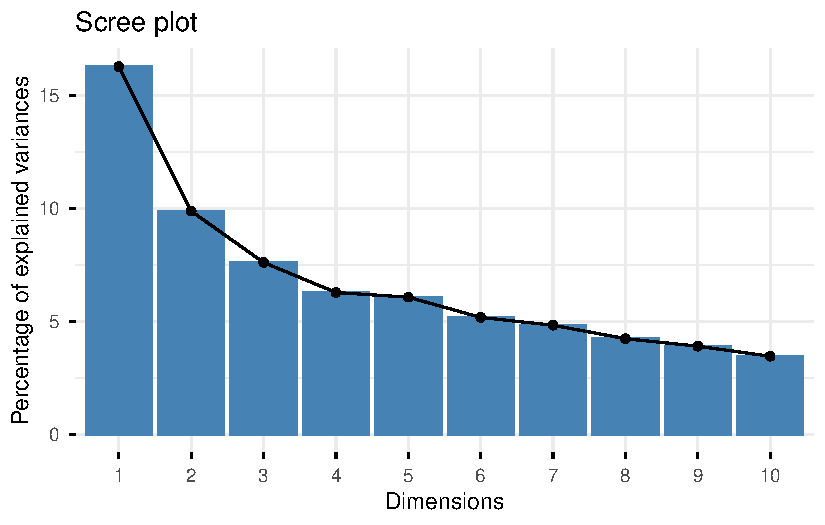
\includegraphics[keepaspectratio]{Explanatory-Data-Analysis_files/figure-pdf/unnamed-chunk-3-1.pdf}}

\begin{Shaded}
\begin{Highlighting}[]
\CommentTok{\#create matrix of raw PC scores (chosen from scree plot)}
\NormalTok{pc\_scores }\OtherTok{\textless{}{-}} \FunctionTok{as.data.frame}\NormalTok{(pca}\SpecialCharTok{$}\NormalTok{x[, }\DecValTok{1}\SpecialCharTok{:}\DecValTok{10}\NormalTok{])}

\CommentTok{\#add response variable (mean\_gi) into new dataframe}
\NormalTok{pc\_data }\OtherTok{\textless{}{-}}\NormalTok{ pc\_scores }\SpecialCharTok{\%\textgreater{}\%}
              \FunctionTok{mutate}\NormalTok{(}\AttributeTok{mean\_gi =}\NormalTok{ predictors}\SpecialCharTok{$}\NormalTok{mean\_gi)}

\CommentTok{\#set priors for brm }
\NormalTok{priors\_pca }\OtherTok{\textless{}{-}} \FunctionTok{c}\NormalTok{(}
  \FunctionTok{prior}\NormalTok{(}\FunctionTok{normal}\NormalTok{(}\DecValTok{0}\NormalTok{, }\DecValTok{1}\NormalTok{), }\AttributeTok{class =} \StringTok{"b"}\NormalTok{),}
  \FunctionTok{prior}\NormalTok{(}\FunctionTok{normal}\NormalTok{(}\FloatTok{6.5}\NormalTok{, }\DecValTok{2}\NormalTok{), }\AttributeTok{class =} \StringTok{"Intercept"}\NormalTok{), }\CommentTok{\#mean mean\_gi is \textasciitilde{}6.5}
  \FunctionTok{prior}\NormalTok{(}\FunctionTok{student\_t}\NormalTok{(}\DecValTok{3}\NormalTok{, }\DecValTok{0}\NormalTok{, }\DecValTok{2}\NormalTok{), }\AttributeTok{class =} \StringTok{"sigma"}\NormalTok{))}

\CommentTok{\#run brm model}
\NormalTok{model\_pca }\OtherTok{\textless{}{-}} \FunctionTok{brm}\NormalTok{(mean\_gi }\SpecialCharTok{\textasciitilde{}}\NormalTok{ .,}
                 \AttributeTok{data =}\NormalTok{ pc\_data,}
                 \AttributeTok{family =} \FunctionTok{gaussian}\NormalTok{(),}
                 \AttributeTok{prior =}\NormalTok{ priors\_pca,}
                 \AttributeTok{chains =} \DecValTok{4}\NormalTok{, }\AttributeTok{iter =} \DecValTok{4000}\NormalTok{, }\AttributeTok{warmup =} \DecValTok{2000}\NormalTok{,}
                 \AttributeTok{cores =} \DecValTok{4}\NormalTok{)}
\end{Highlighting}
\end{Shaded}

\begin{verbatim}
Compiling Stan program...
\end{verbatim}

\begin{verbatim}
Trying to compile a simple C file
\end{verbatim}

\begin{verbatim}
Running /Library/Frameworks/R.framework/Resources/bin/R CMD SHLIB foo.c
using C compiler: ‘Apple clang version 17.0.0 (clang-1700.6.3.2)’
using SDK: ‘MacOSX26.2.sdk’
clang -arch arm64 -std=gnu2x -I"/Library/Frameworks/R.framework/Resources/include" -DNDEBUG   -I"/Library/Frameworks/R.framework/Versions/4.5-arm64/Resources/library/Rcpp/include/"  -I"/Library/Frameworks/R.framework/Versions/4.5-arm64/Resources/library/RcppEigen/include/"  -I"/Library/Frameworks/R.framework/Versions/4.5-arm64/Resources/library/RcppEigen/include/unsupported"  -I"/Library/Frameworks/R.framework/Versions/4.5-arm64/Resources/library/BH/include" -I"/Library/Frameworks/R.framework/Versions/4.5-arm64/Resources/library/StanHeaders/include/src/"  -I"/Library/Frameworks/R.framework/Versions/4.5-arm64/Resources/library/StanHeaders/include/"  -I"/Library/Frameworks/R.framework/Versions/4.5-arm64/Resources/library/RcppParallel/include/"  -I"/Library/Frameworks/R.framework/Versions/4.5-arm64/Resources/library/rstan/include" -DEIGEN_NO_DEBUG  -DBOOST_DISABLE_ASSERTS  -DBOOST_PENDING_INTEGER_LOG2_HPP  -DSTAN_THREADS  -DUSE_STANC3 -DSTRICT_R_HEADERS  -DBOOST_PHOENIX_NO_VARIADIC_EXPRESSION  -D_HAS_AUTO_PTR_ETC=0  -include '/Library/Frameworks/R.framework/Versions/4.5-arm64/Resources/library/StanHeaders/include/stan/math/prim/fun/Eigen.hpp'  -D_REENTRANT -DRCPP_PARALLEL_USE_TBB=1   -I/opt/R/arm64/include    -fPIC  -falign-functions=64 -Wall -g -O2  -c foo.c -o foo.o
In file included from <built-in>:1:
In file included from /Library/Frameworks/R.framework/Versions/4.5-arm64/Resources/library/StanHeaders/include/stan/math/prim/fun/Eigen.hpp:22:
In file included from /Library/Frameworks/R.framework/Versions/4.5-arm64/Resources/library/RcppEigen/include/Eigen/Dense:1:
In file included from /Library/Frameworks/R.framework/Versions/4.5-arm64/Resources/library/RcppEigen/include/Eigen/Core:19:
/Library/Frameworks/R.framework/Versions/4.5-arm64/Resources/library/RcppEigen/include/Eigen/src/Core/util/Macros.h:679:10: fatal error: 'cmath' file not found
  679 | #include <cmath>
      |          ^~~~~~~
1 error generated.
make: *** [foo.o] Error 1
\end{verbatim}

\begin{verbatim}
Start sampling
\end{verbatim}

\begin{Shaded}
\begin{Highlighting}[]
\FunctionTok{summary}\NormalTok{(model\_pca) }\CommentTok{\#PC1, PC3, and PC6 are significant!}
\end{Highlighting}
\end{Shaded}

\begin{verbatim}
 Family: gaussian 
  Links: mu = identity 
Formula: mean_gi ~ PC1 + PC2 + PC3 + PC4 + PC5 + PC6 + PC7 + PC8 + PC9 + PC10 
   Data: pc_data (Number of observations: 90) 
  Draws: 4 chains, each with iter = 4000; warmup = 2000; thin = 1;
         total post-warmup draws = 8000

Regression Coefficients:
          Estimate Est.Error l-95% CI u-95% CI Rhat Bulk_ESS Tail_ESS
Intercept     6.44      0.24     5.96     6.92 1.00    16308     4948
PC1           0.79      0.10     0.58     0.99 1.00    15307     5830
PC2           0.20      0.13    -0.06     0.46 1.00    17210     6387
PC3          -0.40      0.16    -0.70    -0.09 1.00    17137     6017
PC4           0.02      0.17    -0.30     0.35 1.00    16521     6056
PC5           0.26      0.17    -0.06     0.59 1.00    18312     5639
PC6          -0.38      0.18    -0.74    -0.02 1.00    18988     5877
PC7           0.17      0.19    -0.20     0.54 1.00    17749     5772
PC8           0.06      0.20    -0.33     0.46 1.00    16340     5973
PC9          -0.35      0.21    -0.76     0.07 1.00    18461     5420
PC10          0.03      0.22    -0.40     0.46 1.00    19615     6217

Further Distributional Parameters:
      Estimate Est.Error l-95% CI u-95% CI Rhat Bulk_ESS Tail_ESS
sigma     2.30      0.19     1.98     2.71 1.00    11745     6099

Draws were sampled using sampling(NUTS). For each parameter, Bulk_ESS
and Tail_ESS are effective sample size measures, and Rhat is the potential
scale reduction factor on split chains (at convergence, Rhat = 1).
1 / 4000 [ 50%]  (Sampling)
Chain 3: Iteration: 2400 / 4000 [ 60%]  (Sampling)
Chain 2: Iteration: 2400 / 4000 [ 60%]  (Sampling)
Chain 1: Iteration: 3200 / 4000 [ 80%]  (Sampling)
Chain 4: Iteration: 2400 / 4000 [ 60%]  (Sampling)
Chain 3: Iteration: 2800 / 4000 [ 70%]  (Sampling)
Chain 2: Iteration: 2800 / 4000 [ 70%]  (Sampling)
Chain 1: Iteration: 3600 / 4000 [ 90%]  (Sampling)
Chain 4: Iteration: 2800 / 4000 [ 70%]  (Sampling)
Chain 3: Iteration: 3200 / 4000 [ 80%]  (Sampling)
Chain 2: Iteration: 3200 / 4000 [ 80%]  (Sampling)
Chain 1: Iteration: 4000 / 4000 [100%]  (Sampling)
Chain 1: 
Chain 1:  Elapsed Time: 0.054 seconds (Warm-up)
Chain 1:                0.054 seconds (Sampling)
Chain 1:                0.108 seconds (Total)
Chain 1: 
Chain 4: Iteration: 3200 / 4000 [ 80%]  (Sampling)
Chain 3: Iteration: 3600 / 4000 [ 90%]  (Sampling)
Chain 2: Iteration: 3600 / 4000 [ 90%]  (Sampling)
Chain 4: Iteration: 3600 / 4000 [ 90%]  (Sampling)
Chain 3: Iteration: 4000 / 4000 [100%]  (Sampling)
Chain 3: 
Chain 3:  Elapsed Time: 0.052 seconds (Warm-up)
Chain 3:                0.055 seconds (Sampling)
Chain 3:                0.107 seconds (Total)
Chain 3: 
Chain 2: Iteration: 4000 / 4000 [100%]  (Sampling)
Chain 2: 
Chain 2:  Elapsed Time: 0.056 seconds (Warm-up)
Chain 2:                0.057 seconds (Sampling)
Chain 2:                0.113 seconds (Total)
Chain 2: 
Chain 4: Iteration: 4000 / 4000 [100%]  (Sampling)
Chain 4: 
Chain 4:  Elapsed Time: 0.053 seconds (Warm-up)
Chain 4:                0.056 seconds (Sampling)
Chain 4:                0.109 seconds (Total)
Chain 4: 
\end{verbatim}

explain why we switch to skew\_normal family (include pp\_checks and
loos)

\begin{Shaded}
\begin{Highlighting}[]
\CommentTok{\#posterior predictive check }
\FunctionTok{pp\_check}\NormalTok{(model\_pca) }\CommentTok{\#mostly fits well, doesn\textquotesingle{}t account for bump around x=2}
\end{Highlighting}
\end{Shaded}

\begin{verbatim}
Using 10 posterior draws for ppc type 'dens_overlay' by default.
\end{verbatim}

\pandocbounded{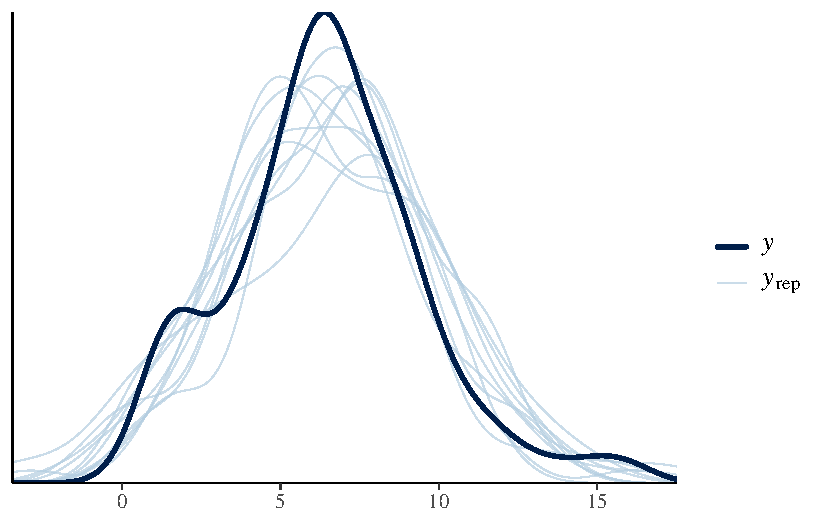
\includegraphics[keepaspectratio]{Explanatory-Data-Analysis_files/figure-pdf/unnamed-chunk-5-1.pdf}}

\begin{Shaded}
\begin{Highlighting}[]
\CommentTok{\#final model }
\NormalTok{model\_pca\_skew }\OtherTok{\textless{}{-}} \FunctionTok{brm}\NormalTok{(mean\_gi }\SpecialCharTok{\textasciitilde{}}\NormalTok{ PC1 }\SpecialCharTok{+}\NormalTok{ PC3 }\SpecialCharTok{+}\NormalTok{ PC6,  }\CommentTok{\# only significant PCs}
                   \AttributeTok{data =}\NormalTok{ pc\_data,}
                   \AttributeTok{family =} \FunctionTok{skew\_normal}\NormalTok{(), }\CommentTok{\#changed to skew\_normal}
                   \AttributeTok{prior =}\NormalTok{ priors\_pca,}
                   \AttributeTok{chains =} \DecValTok{4}\NormalTok{, }\AttributeTok{iter =} \DecValTok{4000}\NormalTok{, }\AttributeTok{warmup =} \DecValTok{2000}\NormalTok{,}
                   \AttributeTok{cores =} \DecValTok{4}\NormalTok{)}
\end{Highlighting}
\end{Shaded}

\begin{verbatim}
Compiling Stan program...
\end{verbatim}

\begin{verbatim}
Trying to compile a simple C file
\end{verbatim}

\begin{verbatim}
Running /Library/Frameworks/R.framework/Resources/bin/R CMD SHLIB foo.c
using C compiler: ‘Apple clang version 17.0.0 (clang-1700.6.3.2)’
using SDK: ‘MacOSX26.2.sdk’
clang -arch arm64 -std=gnu2x -I"/Library/Frameworks/R.framework/Resources/include" -DNDEBUG   -I"/Library/Frameworks/R.framework/Versions/4.5-arm64/Resources/library/Rcpp/include/"  -I"/Library/Frameworks/R.framework/Versions/4.5-arm64/Resources/library/RcppEigen/include/"  -I"/Library/Frameworks/R.framework/Versions/4.5-arm64/Resources/library/RcppEigen/include/unsupported"  -I"/Library/Frameworks/R.framework/Versions/4.5-arm64/Resources/library/BH/include" -I"/Library/Frameworks/R.framework/Versions/4.5-arm64/Resources/library/StanHeaders/include/src/"  -I"/Library/Frameworks/R.framework/Versions/4.5-arm64/Resources/library/StanHeaders/include/"  -I"/Library/Frameworks/R.framework/Versions/4.5-arm64/Resources/library/RcppParallel/include/"  -I"/Library/Frameworks/R.framework/Versions/4.5-arm64/Resources/library/rstan/include" -DEIGEN_NO_DEBUG  -DBOOST_DISABLE_ASSERTS  -DBOOST_PENDING_INTEGER_LOG2_HPP  -DSTAN_THREADS  -DUSE_STANC3 -DSTRICT_R_HEADERS  -DBOOST_PHOENIX_NO_VARIADIC_EXPRESSION  -D_HAS_AUTO_PTR_ETC=0  -include '/Library/Frameworks/R.framework/Versions/4.5-arm64/Resources/library/StanHeaders/include/stan/math/prim/fun/Eigen.hpp'  -D_REENTRANT -DRCPP_PARALLEL_USE_TBB=1   -I/opt/R/arm64/include    -fPIC  -falign-functions=64 -Wall -g -O2  -c foo.c -o foo.o
In file included from <built-in>:1:
In file included from /Library/Frameworks/R.framework/Versions/4.5-arm64/Resources/library/StanHeaders/include/stan/math/prim/fun/Eigen.hpp:22:
In file included from /Library/Frameworks/R.framework/Versions/4.5-arm64/Resources/library/RcppEigen/include/Eigen/Dense:1:
In file included from /Library/Frameworks/R.framework/Versions/4.5-arm64/Resources/library/RcppEigen/include/Eigen/Core:19:
/Library/Frameworks/R.framework/Versions/4.5-arm64/Resources/library/RcppEigen/include/Eigen/src/Core/util/Macros.h:679:10: fatal error: 'cmath' file not found
  679 | #include <cmath>
      |          ^~~~~~~
1 error generated.
make: *** [foo.o] Error 1
\end{verbatim}

\begin{verbatim}
Start sampling
\end{verbatim}

\begin{verbatim}
Warning: There were 1 divergent transitions after warmup. See
https://mc-stan.org/misc/warnings.html#divergent-transitions-after-warmup
to find out why this is a problem and how to eliminate them.
\end{verbatim}

\begin{verbatim}
Warning: Examine the pairs() plot to diagnose sampling problems
\end{verbatim}

\begin{Shaded}
\begin{Highlighting}[]
\FunctionTok{summary}\NormalTok{(model\_pca\_skew) }\CommentTok{\#again, PC1, PC3, and PC6 are significant! }
\end{Highlighting}
\end{Shaded}

\begin{verbatim}
Warning: There were 1 divergent transitions after warmup. Increasing
adapt_delta above 0.8 may help. See
http://mc-stan.org/misc/warnings.html#divergent-transitions-after-warmup
\end{verbatim}

\begin{verbatim}
 Family: skew_normal 
  Links: mu = identity 
Formula: mean_gi ~ PC1 + PC3 + PC6 
   Data: pc_data (Number of observations: 90) 
  Draws: 4 chains, each with iter = 4000; warmup = 2000; thin = 1;
         total post-warmup draws = 8000

Regression Coefficients:
          Estimate Est.Error l-95% CI u-95% CI Rhat Bulk_ESS Tail_ESS
Intercept     6.44      0.24     5.99     6.94 1.00     6416     5389
PC1           0.69      0.08     0.53     0.86 1.00     6194     5105
PC3          -0.46      0.11    -0.68    -0.23 1.00     6596     5497
PC6          -0.32      0.15    -0.62    -0.02 1.00     7932     6256

Further Distributional Parameters:
      Estimate Est.Error l-95% CI u-95% CI Rhat Bulk_ESS Tail_ESS
sigma     2.31      0.19     1.98     2.72 1.00     5908     5625
alpha     4.78      1.88     1.92     9.23 1.00     5456     4509

Draws were sampled using sampling(NUTS). For each parameter, Bulk_ESS
and Tail_ESS are effective sample size measures, and Rhat is the potential
scale reduction factor on split chains (at convergence, Rhat = 1).
teration: 1600 / 4000 [ 40%]  (Warmup)
Chain 4: Iteration: 1600 / 4000 [ 40%]  (Warmup)
Chain 1: Iteration: 2000 / 4000 [ 50%]  (Warmup)
Chain 1: Iteration: 2001 / 4000 [ 50%]  (Sampling)
Chain 2: Iteration: 2000 / 4000 [ 50%]  (Warmup)
Chain 2: Iteration: 2001 / 4000 [ 50%]  (Sampling)
Chain 3: Iteration: 2000 / 4000 [ 50%]  (Warmup)
Chain 3: Iteration: 2001 / 4000 [ 50%]  (Sampling)
Chain 4: Iteration: 2000 / 4000 [ 50%]  (Warmup)
Chain 4: Iteration: 2001 / 4000 [ 50%]  (Sampling)
Chain 1: Iteration: 2400 / 4000 [ 60%]  (Sampling)
Chain 2: Iteration: 2400 / 4000 [ 60%]  (Sampling)
Chain 3: Iteration: 2400 / 4000 [ 60%]  (Sampling)
Chain 2: Iteration: 2800 / 4000 [ 70%]  (Sampling)
Chain 1: Iteration: 2800 / 4000 [ 70%]  (Sampling)
Chain 4: Iteration: 2400 / 4000 [ 60%]  (Sampling)
Chain 3: Iteration: 2800 / 4000 [ 70%]  (Sampling)
Chain 2: Iteration: 3200 / 4000 [ 80%]  (Sampling)
Chain 1: Iteration: 3200 / 4000 [ 80%]  (Sampling)
Chain 3: Iteration: 3200 / 4000 [ 80%]  (Sampling)
Chain 4: Iteration: 2800 / 4000 [ 70%]  (Sampling)
Chain 2: Iteration: 3600 / 4000 [ 90%]  (Sampling)
Chain 1: Iteration: 3600 / 4000 [ 90%]  (Sampling)
Chain 3: Iteration: 3600 / 4000 [ 90%]  (Sampling)
Chain 4: Iteration: 3200 / 4000 [ 80%]  (Sampling)
Chain 2: Iteration: 4000 / 4000 [100%]  (Sampling)
Chain 2: 
Chain 2:  Elapsed Time: 0.267 seconds (Warm-up)
Chain 2:                0.283 seconds (Sampling)
Chain 2:                0.55 seconds (Total)
Chain 2: 
Chain 1: Iteration: 4000 / 4000 [100%]  (Sampling)
Chain 1: 
Chain 1:  Elapsed Time: 0.274 seconds (Warm-up)
Chain 1:                0.294 seconds (Sampling)
Chain 1:                0.568 seconds (Total)
Chain 1: 
Chain 3: Iteration: 4000 / 4000 [100%]  (Sampling)
Chain 3: 
Chain 3:  Elapsed Time: 0.275 seconds (Warm-up)
Chain 3:                0.287 seconds (Sampling)
Chain 3:                0.562 seconds (Total)
Chain 3: 
Chain 4: Iteration: 3600 / 4000 [ 90%]  (Sampling)
Chain 4: Iteration: 4000 / 4000 [100%]  (Sampling)
Chain 4: 
Chain 4:  Elapsed Time: 0.299 seconds (Warm-up)
Chain 4:                0.373 seconds (Sampling)
Chain 4:                0.672 seconds (Total)
Chain 4: 
\end{verbatim}

\begin{Shaded}
\begin{Highlighting}[]
\CommentTok{\#quick check to make sure skew\_normal() is a better fit than gaussian()}
\FunctionTok{pp\_check}\NormalTok{(model\_pca\_skew)}
\end{Highlighting}
\end{Shaded}

\begin{verbatim}
Using 10 posterior draws for ppc type 'dens_overlay' by default.
\end{verbatim}

\pandocbounded{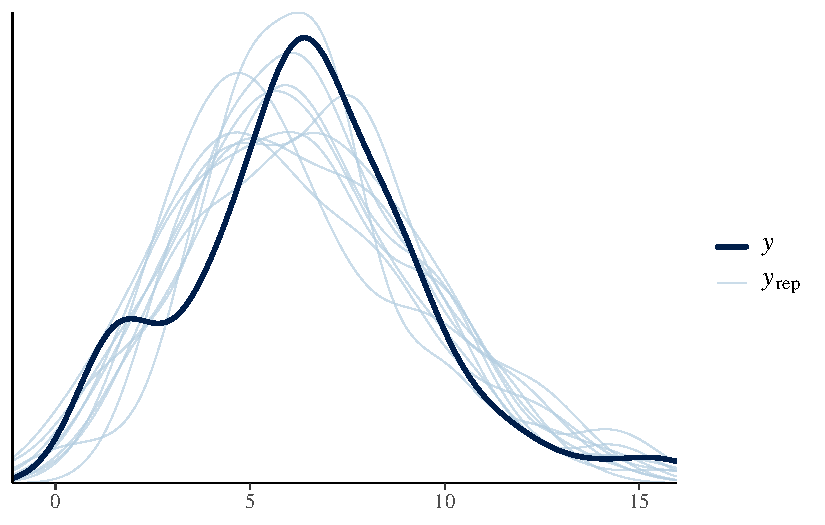
\includegraphics[keepaspectratio]{Explanatory-Data-Analysis_files/figure-pdf/unnamed-chunk-5-2.pdf}}

\begin{Shaded}
\begin{Highlighting}[]
\NormalTok{loo\_gaussian }\OtherTok{\textless{}{-}} \FunctionTok{loo}\NormalTok{(model\_pca)}
\end{Highlighting}
\end{Shaded}

\begin{verbatim}
Warning: Found 1 observations with a pareto_k > 0.7 in model 'model_pca'. We
recommend to set 'moment_match = TRUE' in order to perform moment matching for
problematic observations.
\end{verbatim}

\begin{Shaded}
\begin{Highlighting}[]
\NormalTok{loo\_skew }\OtherTok{\textless{}{-}} \FunctionTok{loo}\NormalTok{(model\_pca\_skew, }\AttributeTok{reloo =} \ConstantTok{TRUE}\NormalTok{)}
\end{Highlighting}
\end{Shaded}

\begin{verbatim}
1 problematic observation(s) found.
The model will be refit 1 times.
\end{verbatim}

\begin{verbatim}

Fitting model 1 out of 1 (leaving out observation 37)
\end{verbatim}

\begin{verbatim}
Start sampling
\end{verbatim}

\begin{Shaded}
\begin{Highlighting}[]
\FunctionTok{loo\_compare}\NormalTok{(loo\_gaussian, loo\_skew)}

\CommentTok{\#what predictors are included in PC1, PC3, and PC6?}
\ControlFlowTok{for}\NormalTok{(pc }\ControlFlowTok{in} \FunctionTok{c}\NormalTok{(}\StringTok{"PC1"}\NormalTok{,}\StringTok{"PC3"}\NormalTok{,}\StringTok{"PC6"}\NormalTok{)) \{ }\CommentTok{\#starts a for loop }
  \FunctionTok{cat}\NormalTok{(}\StringTok{"}\SpecialCharTok{\textbackslash{}n}\StringTok{{-}{-}{-}"}\NormalTok{, pc, }\StringTok{"{-}{-}{-}}\SpecialCharTok{\textbackslash{}n}\StringTok{"}\NormalTok{) }\CommentTok{\#syntax for output: headers for each PC}
  \FunctionTok{cat}\NormalTok{(}\StringTok{"TOP POSITIVE:}\SpecialCharTok{\textbackslash{}n}\StringTok{"}\NormalTok{) }\CommentTok{\#syntax for output: label for the variables with  largest positive loadings for the current PC}
  \FunctionTok{print}\NormalTok{(}\FunctionTok{head}\NormalTok{(}\FunctionTok{sort}\NormalTok{(pca}\SpecialCharTok{$}\NormalTok{rotation[,pc], }\AttributeTok{decreasing =} \ConstantTok{TRUE}\NormalTok{), }\DecValTok{5}\NormalTok{)) }\CommentTok{\#sorts loadings from largest to smallest, keeps top 5 variables }
  \FunctionTok{cat}\NormalTok{(}\StringTok{"TOP NEGATIVE:}\SpecialCharTok{\textbackslash{}n}\StringTok{"}\NormalTok{) }\CommentTok{\#syntax for output: label for the variables with  largest negative loadings for the current PC}
  \FunctionTok{print}\NormalTok{(}\FunctionTok{head}\NormalTok{(}\FunctionTok{sort}\NormalTok{(pca}\SpecialCharTok{$}\NormalTok{rotation[,pc], }\AttributeTok{decreasing =} \ConstantTok{FALSE}\NormalTok{), }\DecValTok{5}\NormalTok{))\} }\CommentTok{\#sorts loadings from largest to smallest, keeps top 5 variables }
\end{Highlighting}
\end{Shaded}

interpret graph (posterior distributions)

\begin{Shaded}
\begin{Highlighting}[]
\CommentTok{\#density curves of each PC showing posterior distributions }
\FunctionTok{mcmc\_areas}\NormalTok{(model\_pca\_skew,}
           \AttributeTok{pars =} \FunctionTok{vars}\NormalTok{(}\FunctionTok{starts\_with}\NormalTok{(}\StringTok{"b\_"}\NormalTok{), }\SpecialCharTok{{-}}\NormalTok{b\_Intercept), }\CommentTok{\#plot regression coefficients and exclude intercept }
           \AttributeTok{prob =} \FloatTok{0.95}\NormalTok{, }\CommentTok{\#shade the 95\% credible interval }
           \AttributeTok{prob\_outer =} \FloatTok{1.0}\NormalTok{) }\SpecialCharTok{+}
  \FunctionTok{geom\_vline}\NormalTok{(}\AttributeTok{xintercept =} \DecValTok{0}\NormalTok{, }\AttributeTok{linetype =} \StringTok{"dashed"}\NormalTok{, }\AttributeTok{color =} \StringTok{"red"}\NormalTok{) }\SpecialCharTok{+} \CommentTok{\#dotted line at x=0 for visual assessment }
  \FunctionTok{theme\_classic}\NormalTok{()}
\end{Highlighting}
\end{Shaded}

\pandocbounded{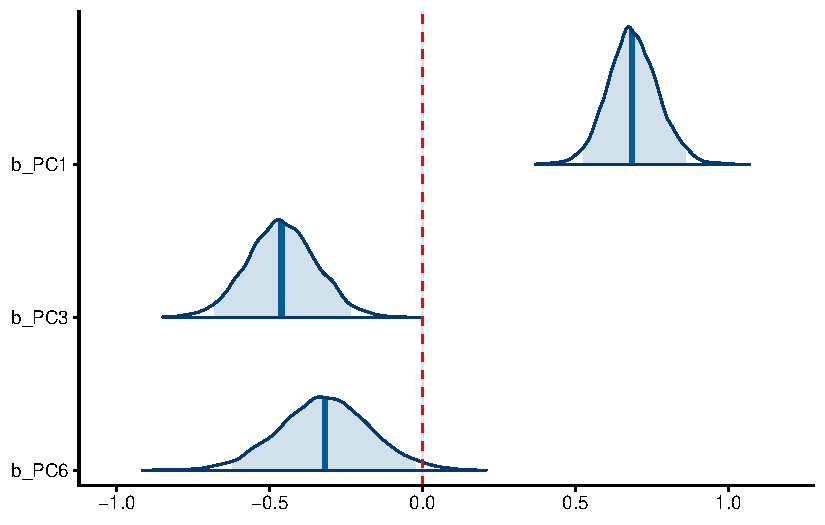
\includegraphics[keepaspectratio]{Explanatory-Data-Analysis_files/figure-pdf/unnamed-chunk-6-1.pdf}}

explain predicted vs observation plot

\begin{Shaded}
\begin{Highlighting}[]
\NormalTok{pc\_data}\SpecialCharTok{$}\NormalTok{fitted }\OtherTok{\textless{}{-}} \FunctionTok{fitted}\NormalTok{(model\_pca\_skew)[, }\StringTok{"Estimate"}\NormalTok{] }\CommentTok{\#posterior mean prediction for each observation}
\NormalTok{pc\_data}\SpecialCharTok{$}\NormalTok{lower  }\OtherTok{\textless{}{-}} \FunctionTok{fitted}\NormalTok{(model\_pca\_skew)[, }\StringTok{"Q2.5"}\NormalTok{] }\CommentTok{\#lower 95\% credible interval}
\NormalTok{pc\_data}\SpecialCharTok{$}\NormalTok{upper  }\OtherTok{\textless{}{-}} \FunctionTok{fitted}\NormalTok{(model\_pca\_skew)[, }\StringTok{"Q97.5"}\NormalTok{] }\CommentTok{\#upper 95\% credible interval}

\CommentTok{\#plot observed vs predicted to see how well the three ecologically meaningful PCs predict gonad index}
\FunctionTok{ggplot}\NormalTok{(pc\_data, }\FunctionTok{aes}\NormalTok{(}\AttributeTok{x =}\NormalTok{ fitted}\SpecialCharTok{/}\DecValTok{100}\NormalTok{, }\AttributeTok{y =}\NormalTok{ mean\_gi}\SpecialCharTok{/}\DecValTok{100}\NormalTok{)) }\SpecialCharTok{+} \CommentTok{\#turn units to \%}
  \FunctionTok{geom\_point}\NormalTok{(}\AttributeTok{color =} \StringTok{"\#466995"}\NormalTok{) }\SpecialCharTok{+} \CommentTok{\#each dot is one observation }
  \FunctionTok{geom\_errorbarh}\NormalTok{(}\FunctionTok{aes}\NormalTok{(}\AttributeTok{xmin =}\NormalTok{ lower, }\AttributeTok{xmax =}\NormalTok{ upper), }\AttributeTok{alpha =} \FloatTok{0.2}\NormalTok{, }\AttributeTok{size =} \FloatTok{0.3}\NormalTok{) }\SpecialCharTok{+} \CommentTok{\#horizontal error bars showing prediction uncertainty}
  \FunctionTok{geom\_abline}\NormalTok{(}\AttributeTok{slope =} \DecValTok{1}\NormalTok{, }\AttributeTok{intercept =} \DecValTok{0}\NormalTok{, }\AttributeTok{linetype =} \StringTok{"dashed"}\NormalTok{, }\AttributeTok{color =} \StringTok{"red"}\NormalTok{) }\SpecialCharTok{+} \CommentTok{\#prediction line }
  \FunctionTok{labs}\NormalTok{(}\AttributeTok{x =} \StringTok{"Predicted Mean GI (\%)"}\NormalTok{, }\AttributeTok{y =} \StringTok{"Observed Mean GI (\%)"}\NormalTok{) }\SpecialCharTok{+}
  \FunctionTok{scale\_x\_continuous}\NormalTok{(}\AttributeTok{limits =} \FunctionTok{c}\NormalTok{(}\DecValTok{0}\NormalTok{,}\FloatTok{0.15}\NormalTok{)) }\SpecialCharTok{+}
  \FunctionTok{scale\_y\_continuous}\NormalTok{(}\AttributeTok{limits =} \FunctionTok{c}\NormalTok{(}\DecValTok{0}\NormalTok{,}\FloatTok{0.2}\NormalTok{)) }\SpecialCharTok{+}
  \FunctionTok{theme\_classic}\NormalTok{()}
\end{Highlighting}
\end{Shaded}

\begin{verbatim}
Warning: `geom_errorbarh()` was deprecated in ggplot2 4.0.0.
i Please use the `orientation` argument of `geom_errorbar()` instead.
\end{verbatim}

\begin{verbatim}
Warning: Using `size` aesthetic for lines was deprecated in ggplot2 3.4.0.
i Please use `linewidth` instead.
i The deprecated feature was likely used in the ggplot2 package.
  Please report the issue at <https://github.com/tidyverse/ggplot2/issues>.
\end{verbatim}

\pandocbounded{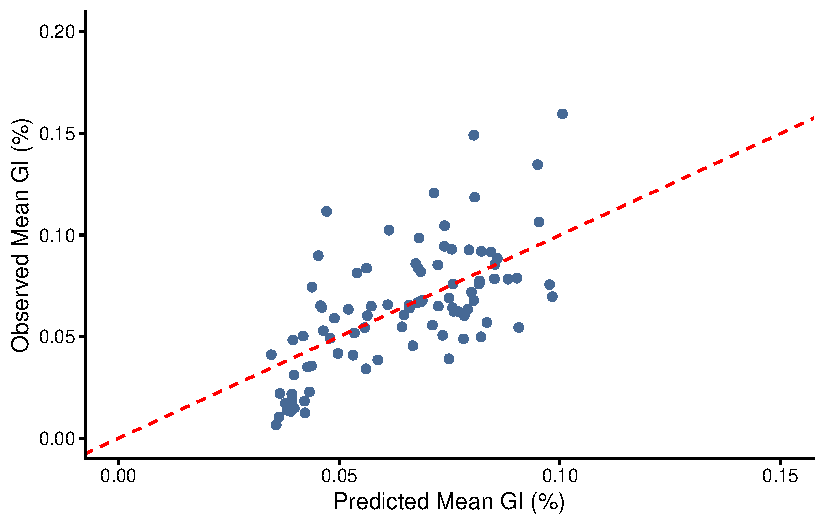
\includegraphics[keepaspectratio]{Explanatory-Data-Analysis_files/figure-pdf/unnamed-chunk-7-1.pdf}}

\begin{Shaded}
\begin{Highlighting}[]
\CommentTok{\#plotting }




\FunctionTok{fviz\_pca\_var}\NormalTok{(}
\NormalTok{  pca,}
  \AttributeTok{col.var =} \StringTok{"contrib"}\NormalTok{,  }\CommentTok{\# color by contribution to the PC axes}
  \AttributeTok{repel =} \ConstantTok{TRUE}\NormalTok{,}
  \AttributeTok{gradient.cols =} \FunctionTok{c}\NormalTok{(}\StringTok{"grey80"}\NormalTok{, }\StringTok{"steelblue"}\NormalTok{, }\StringTok{"darkblue"}\NormalTok{)}
\NormalTok{) }\SpecialCharTok{+}
  \FunctionTok{labs}\NormalTok{(}\AttributeTok{title =} \StringTok{"PCA variable plot"}\NormalTok{)}
\end{Highlighting}
\end{Shaded}

\begin{verbatim}
Warning: `aes_string()` was deprecated in ggplot2 3.0.0.
i Please use tidy evaluation idioms with `aes()`.
i See also `vignette("ggplot2-in-packages")` for more information.
i The deprecated feature was likely used in the factoextra package.
  Please report the issue at <https://github.com/kassambara/factoextra/issues>.
\end{verbatim}

\pandocbounded{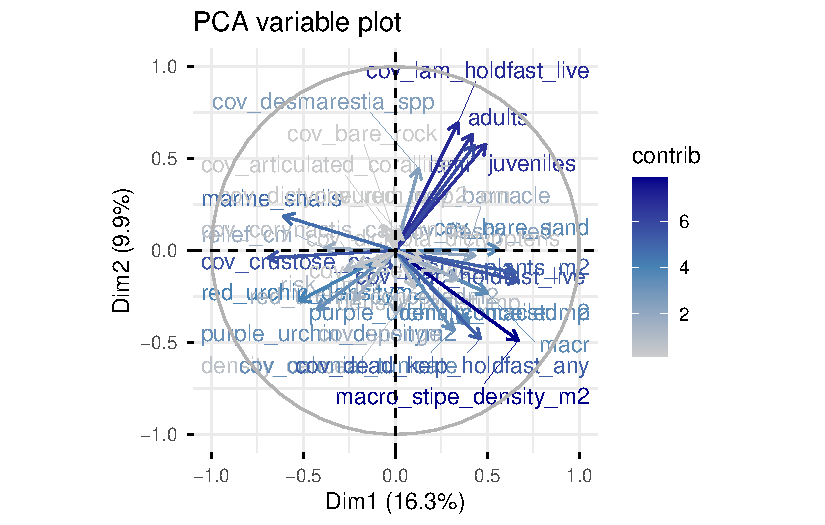
\includegraphics[keepaspectratio]{Explanatory-Data-Analysis_files/figure-pdf/unnamed-chunk-8-1.pdf}}

\section{4. uhhhh - horseshoe?}\label{uhhhh---horseshoe}

\begin{Shaded}
\begin{Highlighting}[]
\CommentTok{\#explain why hand{-}picking is not as honest than PCA? }
\NormalTok{glm }\OtherTok{\textless{}{-}} \FunctionTok{glm}\NormalTok{(mean\_gi }\SpecialCharTok{\textasciitilde{}}\NormalTok{ PC1 }\SpecialCharTok{+}\NormalTok{ PC3 }\SpecialCharTok{+}\NormalTok{ PC6, }\AttributeTok{data =}\NormalTok{ pc\_data)}
\end{Highlighting}
\end{Shaded}





\end{document}
